\documentclass[acmsmall]{acmart}

\usepackage{booktabs} % For formal tables


% \usepackage[ruled]{algorithm2e} % For algorithms

\usepackage{cleveref}
\usepackage{epsfig}
\usepackage{float}
\usepackage{amsmath,amssymb,amsfonts}
\usepackage{algorithm}
\usepackage[noend]{algpseudocode}
\usepackage{bigstrut,multirow}
\usepackage{threeparttable}
\usepackage{subfigure}
\usepackage{url}

% \renewcommand{\algorithmcfname}{ALGORITHM}
% \SetAlFnt{\small}
% \SetAlCapFnt{\small}
% \SetAlCapNameFnt{\small}
% \SetAlCapHSkip{0pt}
% \IncMargin{-\parindent}

% Metadata Information
\acmJournal{TRETS}
\acmVolume{9}
\acmNumber{4}
\acmArticle{11}
\acmYear{2017}
\acmMonth{12}
\acmArticleSeq{11}

%\acmBadgeR[http://ctuning.org/ae/ppopp2016.html]{ae-logo}
%\acmBadgeL[http://ctuning.org/ae/ppopp2016.html]{ae-logo}


% Copyright
%\setcopyright{acmcopyright}
%\setcopyright{acmlicensed}
%\setcopyright{rightsretained}
%\setcopyright{usgov}
\setcopyright{usgovmixed}
%\setcopyright{cagov}
%\setcopyright{cagovmixed}

% DOI
\acmDOI{0000001.0000001}

% Paper history
% \received{February 2007}
% \received{March 2009}
% \received[accepted]{June 2009}


% Document starts
\begin{document}
% Title portion
\title{[DL] A Survey of FPGA Based Neural Network Accelerator} 
% \titlenote{We can add a note to the title}

\author{Kaiyuan Guo, Shulin Zeng, Jincheng Yu, Yu Wang {\scshape and} Huazhong Yang}
% \authornote{This is the corresponding author}
% \orcid{1234-5678-9012-3456}
\affiliation{%
  \institution{Tsinghua University}
  \streetaddress{Tsinghua University}
  \city{Beijing}
  \state{Beijing}
  \postcode{100084}
  \country{China}}
\email{gky15@mails.tsinghua.edu.cn, yu-wang@mail.tsinghua.edu.cn}

% \author{Yiming Hu}
% \authornote{This is the corresponding author}
% \orcid{1234-5678-9012-3456}
% \affiliation{%
%   \institution{Tsinghua University}
%   \streetaddress{Tsinghua University}
%   \city{Beijing}
%   \state{Beijing}
%   \postcode{100084}
%   \country{China}}
% \email{hym16@mails.tsinghua.edu.cn}


%
% The code below should be generated by the tool at
% http://dl.acm.org/ccs.cfm
% Please copy and paste the code instead of the example below. 
%

\begin{abstract}

Recent researches on neural network have shown significant advantage in machine learning over traditional algorithms based on handcrafted features and models. Neural network is now widely adopted in regions like image, speech and video recognition. But the high computation and storage complexity of neural network inference poses great difficulty on its application. CPU platforms are hard to offer enough computation capacity. GPU platforms are the first choice for neural network process because of its high computation capacity and easy to use development frameworks. 

On the other hand, FPGA-based neural network inference accelerator is becoming a research topic. With specifically designed hardware, FPGA is the next possible solution to surpass GPU in speed and energy efficiency. Various FPGA-based accelerator designs have been proposed with software and hardware optimization techniques to achieve high speed and energy efficiency. In this paper, we give an overview of previous work on neural network inference accelerators based on FPGA and summarize the main techniques used. An investigation from software to hardware, from circuit level to system level is carried out to complete analysis of FPGA-based neural network inference accelerator design and serves as a guide to future work. 

\end{abstract}

\begin{CCSXML}
  <ccs2012>
  <concept>
  <concept_id>10010520.10010553.10010562.10010563</concept_id>
  <concept_desc>Computer systems organization~Embedded hardware</concept_desc>
  <concept_significance>500</concept_significance>
  </concept>
  <concept>
  <concept_id>10010520.10010570.10010574</concept_id>
  <concept_desc>Computer systems organization~Real-time system architecture</concept_desc>
  <concept_significance>300</concept_significance>
  </concept>
  </ccs2012>
  \end{CCSXML}
  
  \ccsdesc[500]{Computer systems organization~Embedded hardware}
  \ccsdesc[300]{Computer systems organization~Real-time system architecture}

\end{CCSXML}
%
% End generated code
%


\keywords{FPGA, Neural Network}

% DO NOT use this command unless you want to change
% the default behavior
% \authorsaddresses{Authors' addresses: G.~Zhou, Computer Science
%   Department, College of William and Mary, 104 Jameson Rd,
%   Williamsburg, PA 23185, US, \path{gzhou@wm.edu}; V.~B\'eranger,
%   Inria Paris-Rocquencourt, Rocquencourt, France; A.~Patel, Rajiv
%   Gandhi University, Rono-Hills, Doimukh, Arunachal Pradesh, India;
%   H.~Chan, Tsinghua University, 30 Shuangqing Rd, Haidian Qu, Beijing
%   Shi, China; T.~Yan, Eaton Innovation Center, Prague, Czech Republic;
%   T.~He, C.~Huang, J.~A.~Stankovic University of Virginia, School of
%   Engineering Charlottesville, VA 22903, USA; T. F. Abdelzaher,
%   (Current address) NASA Ames Research Center, Moffett Field,
%   California 94035.}

\maketitle

% The default list of authors is too long for headers.
\renewcommand{\shortauthors}{K. Guo et al.}

\section{Introduction}\label{sec:introduction}

Recent research on Neural Network (NN) is showing great improvement over traditional algorithms in computer vision. Various network models, like convolutional neural network (CNN), recurrent neural network (RNN), have been proposed for image, video, and speech process. CNN~\cite{krizhevsky2012imagenet} improves the top-5 image classification accuracy on ImageNet~\cite{ILSVRC15} dataset from 73.8\% to 84.7\% and further helps improve object detection~\cite{girshick2014rich} with its outstanding ability in feature extraction. RNN~\cite{hannun2014deep} achieves state-of-the-art word error rate on speech recognition. In general, NN features a high fitting ability to a wide range of pattern recognition problems. This makes NN a promising candidate to many artificial intelligence applications.

But the computation and storage complexity of NN models are high. The research on NN is also increasing the size of NN models. The largest neural network model for an $224\times224$ image classification requires upto 39 billion floating point operations (FLOP) and more than 500MB model parameters~\cite{simonyan2014very}. As the computation complexity is propotional to the input image size, processing images with higher resolutions may need more than 100 billion operations.

Traditional hardware platforms are not suitable for neural network process. A common CPU can perform 10-100G FLOP per second, and the power efficieny is usually below 1GOPs/W. So CPUs neither meet the high performance requirements in cloud applications nor the low power requiremetns in mobile applications. In contrast, GPUs offer upto 10TOP/s peak performance and is a good choice for high performance neural network applications. Development frameworks like Caffe~\cite{jia2014caffe} and Tensorflow~\cite{abadi2016tensorflow} also offers easy-to-use interfaces which makes GPU the first choice of neural network acceleration. But GPUs are power consuming and thus not suitable for mobile applications.

On the other hand, FPGA is becoming a candidate to implement energy efficient neural network accelerator. With a specific hardware design, FPGAs are able to implement high parallelism and make use of the properties of neural network computation to remove unecessary logic. Therefore FPGAs are possible to achieve higher energy efficieny compared with CPU and GPU. 

But FPGA based accelerator designs are still faced with two problems:
\begin{itemize}
    \item Current FPGAs usually support working frequency at 100-300MHz, which is much less than CPU and GPU. The FPGA's logic overhead for reconfigurability also reduces the overall system performance. Straight forward design on FPGA is hard to achieve high performance and high energy efficiency.
    \item Implementation of neural networks on FPGAs is much harder than that on CPUs or GPUs. Development framework like Caffe and Tensorflow for CPU and GPU is needed for FPGA.
\end{itemize}
 
Many researches on the above two problems have been carried out for energy efficient and flexible FPGA based neural network accelerator. In this paper, we summarize the techniques proposed in these work. Specifically, we will introduce the techiques from the following aspects:
\begin{itemize}
    \item We investigate current techniques for high performance and energy efficient neural network accelerator designs. Techniques in both software level and hardware level are evaluated.
    \item We investigate state-of-the-art automatic design methods of FPGA based neural network accelerators. 
\end{itemize}

The rest part of this paper is organized as follows:

\section{Preliminary}\label{sec:preliminary}

\rev{Before discussing the system design for neural network acceleration, we first introduce the basic concepts of neural networks and the basic components of an FPGA-based accelerator design.}

\subsection{Neural Network}

\begin{figure}[ht]
    \centering
    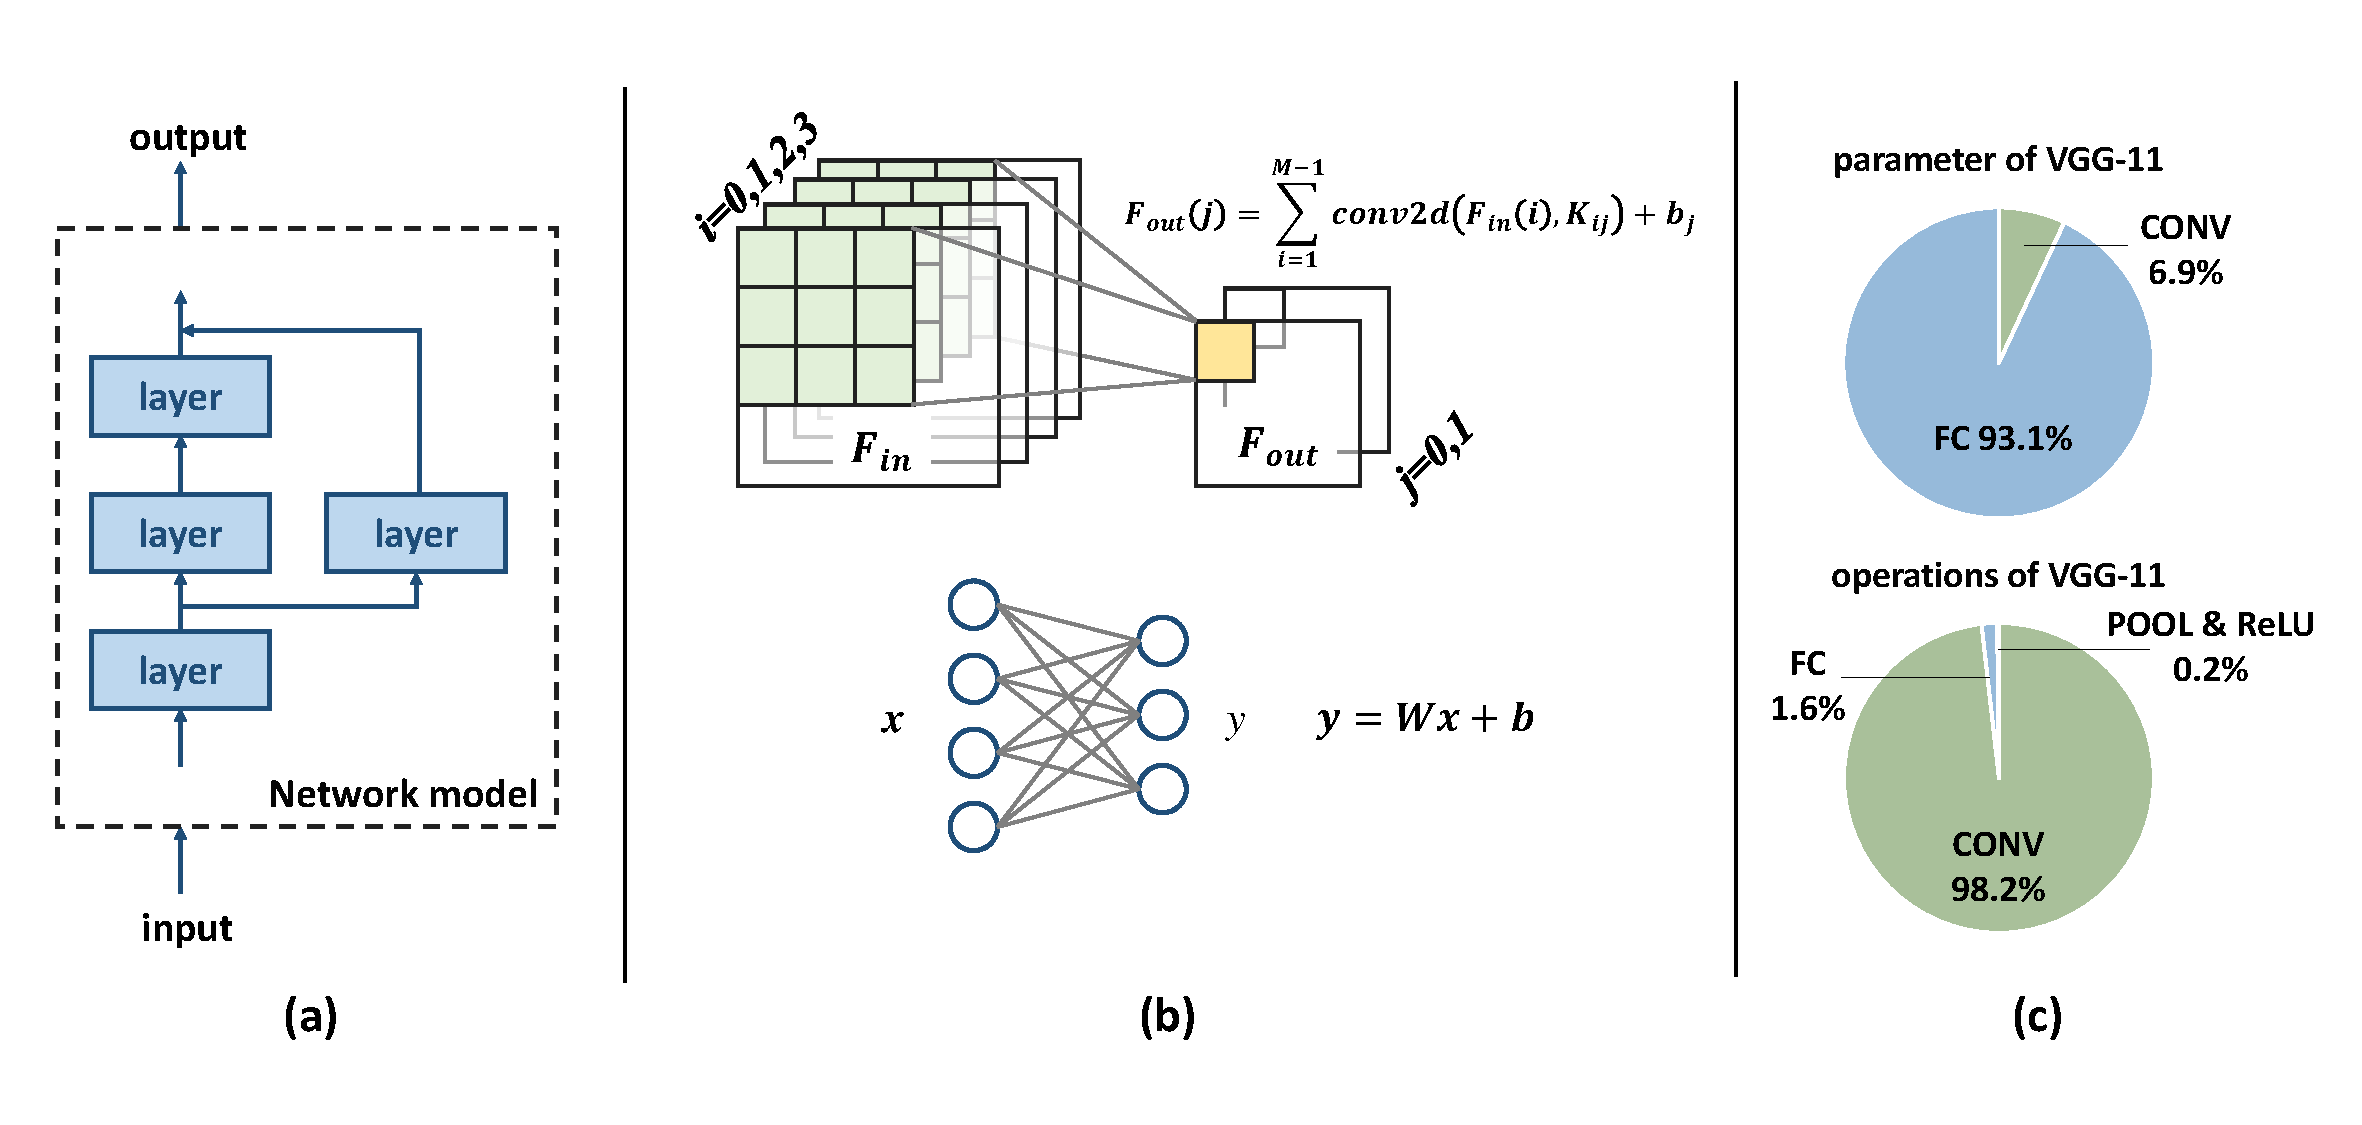
\includegraphics[width=1.0\columnwidth]{fig/cnn_preliminary.pdf}
    \caption{\rev{(a) Computation graph of a neural network model. (b) CONV and FC layers in NN model. (c) CONV and FC layers dominates the computation and parameter of a NN model.}}
    \label{fig:cnn_preliminary}
\end{figure}

\rev{In this section, we introduce the basic functions in a neural network. A neural network model can be described as a directed graph shown in Figure~\ref{fig:cnn_preliminary}(a). Each vertex of the graph denotes a layer which conducts operations on data from a previous layer or input and generates results to the next layer or output.

Convolution (CONV) layers and fully connected (FC) layers are two common types of layers in NN models. The functions of these two layers are shown in Figure~\ref{fig:cnn_preliminary}(b). CONV layers conduct 2D convolutions on a set of input feature maps $F_{in}$ and add the results to get output feature maps $F_{out}$. FC layers receives a feature vector as input and conduct matrix-vector multiplications.

Besides CONV and FC layers, NN layers also have pooling, ReLU~\cite{krizhevsky2012imagenet}, concat~\cite{szegedy2015going}, element-wise~\cite{he2016deep} and other types of layers. But these layers contributes little to the computation and storage requirement of a neural network model. Figure~\ref{fig:cnn_preliminary}(c) shows the distribution of parameter and operations in the VGG-11 model~\cite{simonyan2014very}. CONV and FC layers together contributes more than 99\% of the network's parameters and operations. So most of the neural network acceleration systems focus on these two types of layers.
}

\subsection{FPGA-based Accelerator}

\rev{In recent years, FPGA is becoming a promising solution for accelerating certain algorithms. Compared with CPU, GPU, and DSP platforms, for which the software and hardware are designed independently, FPGA enables the developers to implement only the necessary logic in hardware according to the target algorithm. By eliminating the redundancy in general hardware platforms, FPGAs are able to achieve higher efficiency. Application specific integrated circuits (ASICs) based solutions achieves even higher efficiency, but requires much longer development cycle and higher cost. 

\begin{figure}[ht]
    \centering
    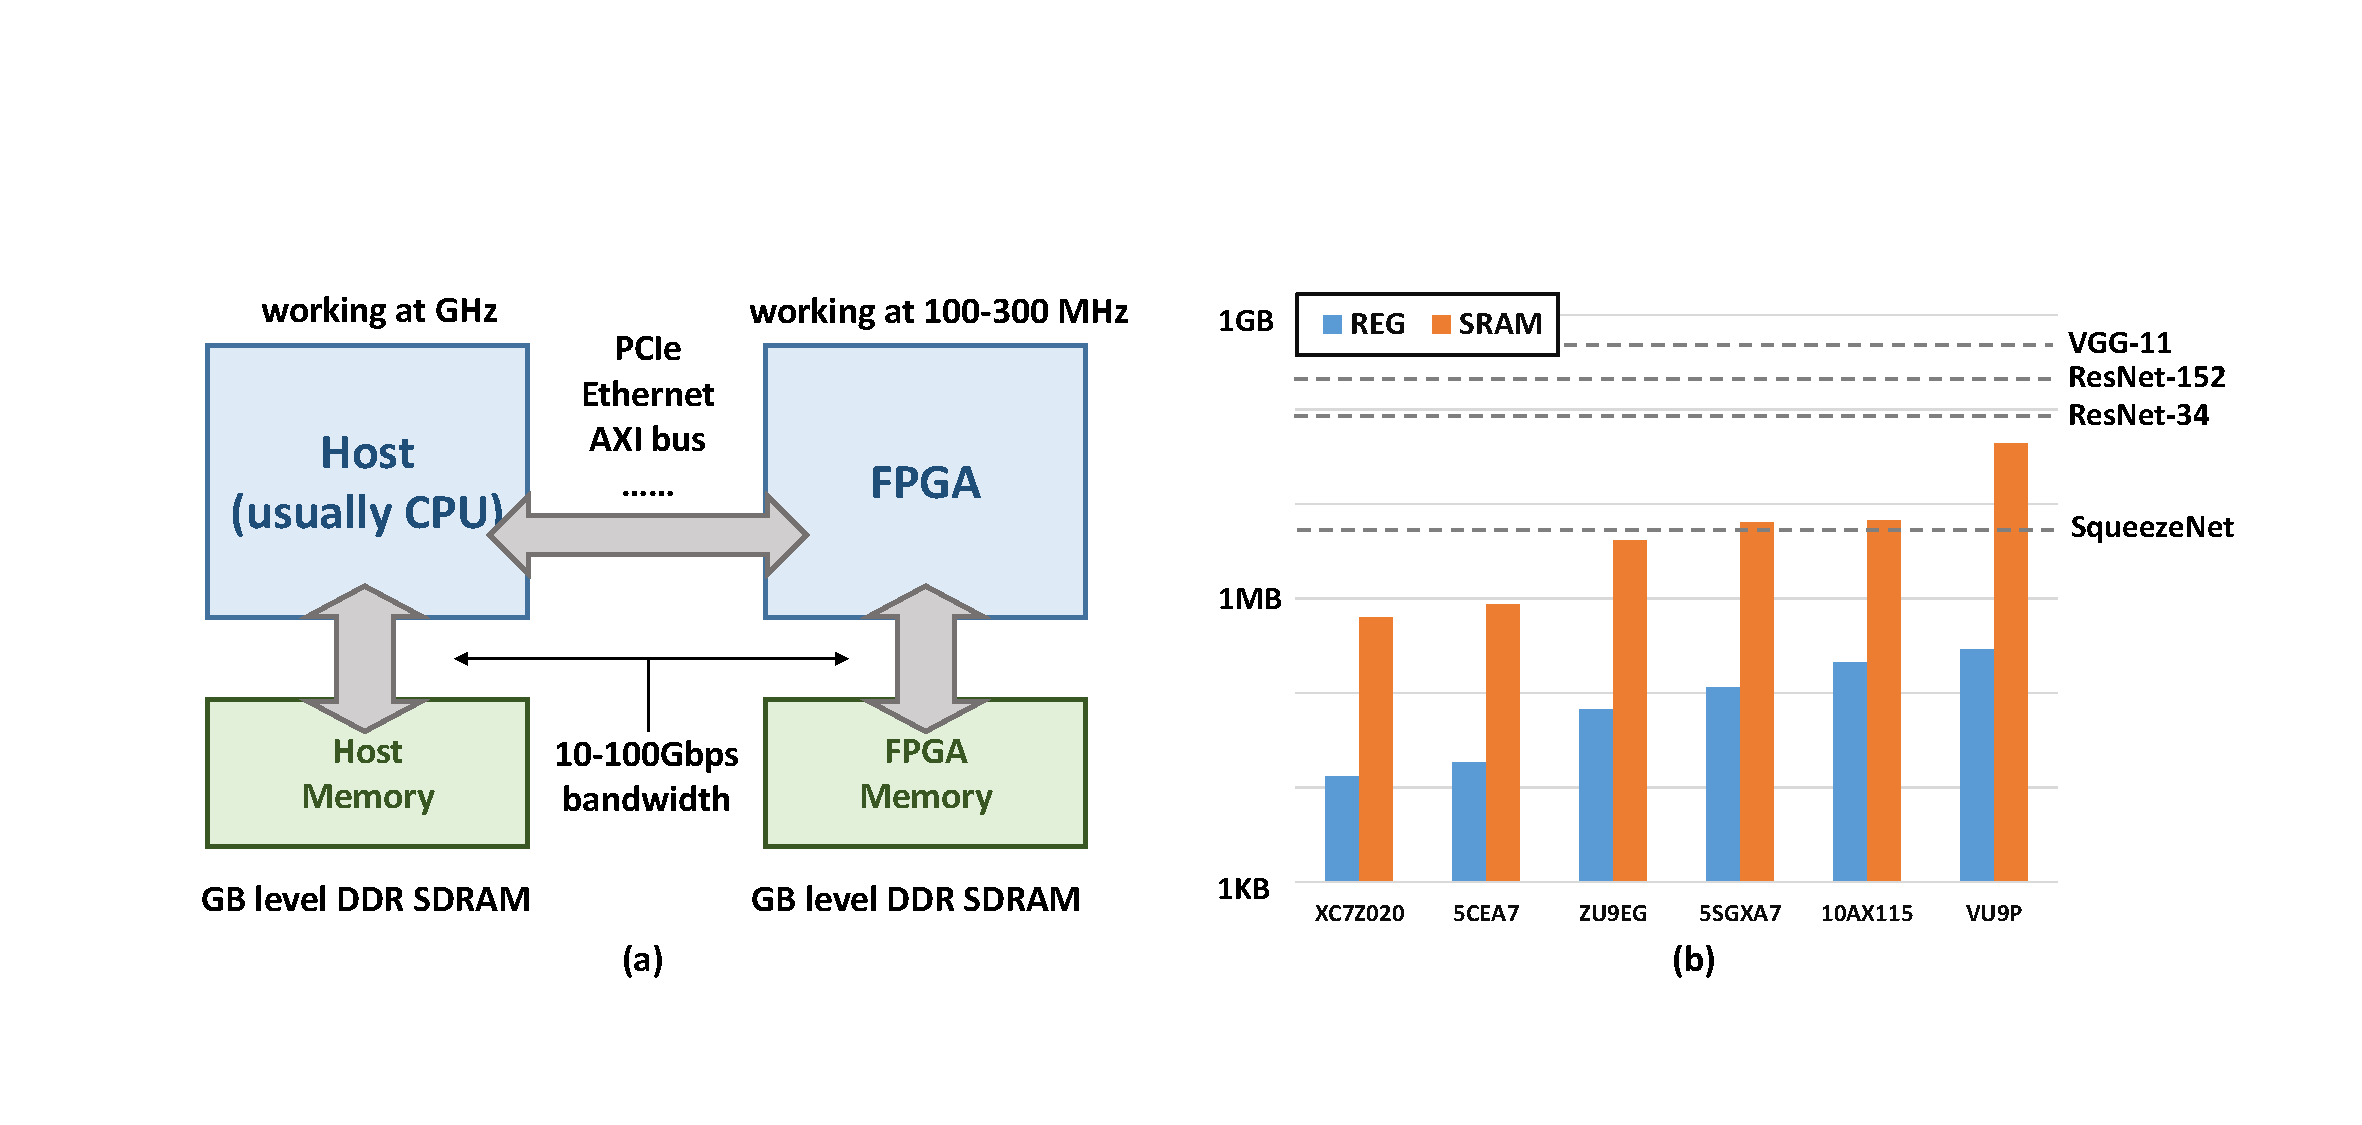
\includegraphics[width=0.8\columnwidth]{fig/fpga_preliminary.pdf}
    \caption{\rev{(a) A typical structure of an FPGA based NN accelerator. (b) Comparison between NN model size and the storage on different FPGA chips.}}
    \label{fig:fpga_preliminary}
\end{figure}

For FPGA-based neural network accelerator, a typical architecture of the system is shown in Figure~\ref{fig:fpga_preliminary}(a). The system usually consists of a CPU host and an FPGA part. A pure FPGA chip usually works with a host PC/server through PCIe connections. SoC platforms (like the Xilinx Zynq Series) and Intel HARPv2~\cite{gupta2016accelerating} platform integrates the host and the FPGA in the same chip or package. Both the host and the FPGA can work with their own external memory and access each others' memory through the connection. Most of the designs implements NN accelerator on the FPGA part and controls the 
acceleartor with the software on the host.

Typical FPGA chips implement large on-chip storage units like registers and SRAMs, but still too small compared with NN models as shown in Figure~\ref{fig:fpga_preliminary}(b). Common models implement 100-1000MB parameters while the largest available FPGA chip implements <50MB on-chip SRAM. This requires that external memory like DDR SDRAM is needed. The bandwidth and power consumption of DDR limits the system performance.

Compared with storage, the computation capacity of FPGA is relatively higher. Common FPGAs implements hundreds to thousands of DSP units, each of which can compute $18\times 27$ or $18\times 19$, achieving upto 10TFLOP/s (floating point operations per second) on the largest FPGAs. But for low-end FPGAs like Xilinx XC7Z020, this number is reduced to 20GFLOP/s, which is hard to support real-time video processing for applications on mobile platforms. 

Even faced with the above challenges, researchers have proposed a series of optimization methods from algorithm to architecture to design high performance NN accelerators on FPGA, which will be discussed in the following sections of this paper.}

\section{Design Methodology}\label{sec:design_method}

Before going into the details of the techniques used for neural network accelerators, we first give an overview of the design methodology. In general, the design target of a neural network processing system includes the following aspects: high model accuracy, high throughput, lower latency, and high energy efficiency.

\rev{A larger neural network model usually results in a higher model accuracy. This means it is possible to tradeoff between the model accuracy and the hardware performance. Neural network researchers are designing more effcient network models from AlexNet~\cite{krizhevsky2012imagenet} to ResNet~\cite{he2016deep}, SqueezeNet~\cite{iandola2016squeezenet} and MobileNet~\cite{Howard2017MobileNets}. The main differences between these networks are the size of and the connections between each layer. The basic operations are the same and hardly affect the hardware design. Other methods try to achieve the tradeoff by optimizing existing NN models. Most of these methods are hardware oriented and will be discussed in detail in section~\ref{sec:software}.}

The throughput of a neural network processing system can be expressed by equation~\ref{eqt:throughput}. With a certain FPGA chip, the on-chip resource is limited. Increasing the peak performance means to reduce the size of each computation unit and increase the working frequency. Reducing the size of computation units can be achieved by simplifying the basic operations in neural network model, which may hurt the model accuracy and requires hardware-software co-design. Increasing working frequency, on the other hand is pure hardware design work. A high utilization ratio is kept by reasonable parallelism implementation and efficient memory system. Most of this part is affected by hardware design. But model compression can also reduce the storage requirment of a neural network model and benefits the memory system.
\begin{equation}\label{eqt:throughput}
    throughput = \frac{peak\_performance \times utilization}{workload}
\end{equation}

Energy efficiency is evaluated by the number of operations (multiplication or addition in this case) executed with unit energy cost. Given a certain network model, the energy efficiency of a neural network processing system is inversely proportional to the energy cost, which is expressed in equation~\ref{eqt:energy}. The energy cost comes from 2 parts: computation and memory access. 
\begin{equation}\label{eqt:energy}
    E_{total} = N_{effect\_op}\times E_{unit\_op} + N_{mem\_access}\times E_{unit\_mem\_access}
\end{equation}

The first item in equation~\ref{eqt:energy} is the energy cost for computation. This part is greatly affected by model compression. Model compression methods can reduce the actual number of operations ($N_{effect\_op}$) to be executed on hardware and simplify the operations to reduce the unit energy cost of a single operation ($E_{unit\_op}$). Given an FPGA chip, $E_{unit\_op}$ is also affected by its hardware implementation. The second item in equation~\ref{eqt:energy} is the energy cost for memory access. The number of memory access $N_{mem\_access}$ is affected by the memory system and scheduling method. The energy for each memory access can be reduced by model compression methods by using a narrower data bit-width. 

From the analysis of throughput and energy, we see that neural network accelerator involves software-hardware co-design. In the following sections, we will introduce previous work in software and hardware level respectively.


\section{Software Design: Model Compression}\label{sec:software}

As introduced in section~\ref{sec:design_method}, the design of energy efficient and high performacne neural network accelerator involves software and hardware co-design. In this section, we investigate the software level network model compression methods. Many researches on this topic have been proposed to reduce the number of weights or reduce the number of bitwidth for the neurons and weights, which helps reudce the computation and storage complexity. But these methods can also sacrifice the model accuracy. The trade-off between model compression and model accuracy loss is discussed in this section.

\subsection{Data Quantization}\label{sec:software:quant}
One of the most commonly used method for model compression is the quantization on the weights and neurons. The neurons and weights of a neural network is usually represented by floating point data in common developing frameworks. Recent work try to replace this representation with low-bit fixed-point data or even a small set of trained values. On one hand, using less bits for each neuron or weight helps reduce the bandwidth and storage requirement of the neural network processing system. On the other hand, using a simplified representation reduce the hardware cost for each operation. The benefit on hardware will be discussed in detail in section~\ref{sec:hardware}. Two kinds of quantization methods are discussed in this section: linear quantization and non-linear quantization.

\subsubsection{Linear Quantization}
Linear quantization finds the nearest fixed-point representation of each weight and neuron. The problem of this method is that the dynamic range of floating point data greatly exceeds that for fixed point data. Most of the weights and neurons will suffer from overflow or underflow. Qiu, et al.~\cite{qiu2016going} finds that the dynamic range of the weights and neurons in a single layer is much more limited and differs across different layers. Therefore they assign different fractional bit-widths to the weights and neurons in different layers. To decide the fractional bit-width of a set of data, i.e. the neurons or weights of a layer, the data distribution is first analyzed. A set of possible fractional bit-widths are chosen as candidate solutions. Then the solution with the best model performance on training data set is chosen. In~\cite{qiu2016going}, the optimized solution of a network is chosen layer by layer to avoid an exponential design space exploration. Guo, et al.~\cite{guo2017angel} further improves this method by fine tuning the model after the fraction bit-width of all the layers are fixed.

The method of choosing certain fractional bit-width equals to scale the data with a scaling factor of $2^k$. Li, et al.~\cite{li2016ternary} scales the weights with trained parameter $W^l$ for each layer and quantize the weights with 2-bit data, representing $W^l$, 0 and $-W^l$. The neurons in this work is not quantized. So the the network still implements 32-bit floating point operations. Zhou, et al.~\cite{zhou2016dorefa} further quantize the weights of a layer with only 1 bit to $\pm s$, where $s=E(|w^l|)$ is the expectation of the absolute value of the weights of this layer. Linear quantization is also applied to the neurons in this work.

\subsubsection{Non-linear Quantization}
Compared with linear quantization, non-linear quantization independently assigns values to different binary code. The translation from a non-linear quantized code to its corresponding value is thus a look-up table. This kind of methods helps further reduce the bit-width used for each neuron or weight. Chen, et al.~\cite{chen2015compressing} assign each of the weight to an item in the look-up table by a pre-defined hash function and train the values in look-up table. Han et al.~\cite{han2015deep} assigns the values in look-up table to the weights by clustering the weights of a trained model. Each look-up table value is set as the cluster center and further fine-tuned with training data set. This method is able to compress the weights of state-of-the-art CNN models to 4-bit without accuracy loss. Zhu, et al.~\cite{zhu2016trained} propose the ternary quantized network where all the weights of a layer are quantized to three values: $W^n$, 0, and $W^p$. Both the quantized value and the correspondance between weights and look-up table are trained. This method sacrifices less than $2\%$ accuracy loss on ImageNet data set on state-of-the-art network models. The weight bit-width is reduced from 32-bit to 2-bit, which means about $16\times$ model size compression.

\subsubsection{Comparison}
We compare different quantization methods in Figure~\ref{fig:quantization}. The labels describe the experiments as $BW_{weight}\times BW_{neurons}$ and network name. The "(FT)" denotes that the network is fine-tuned after a linear quantization. Comparing different methods on different models is a little bit unfair. But it still gives some insights. For linear quantization, 8-bit is a clear bound to ensure negligible accuracy loss. With 6 or less bits, using fine-tune or even training each weight from the beginning, will cause obvious accuracy degradation.

\begin{figure}[h]
    \centering
    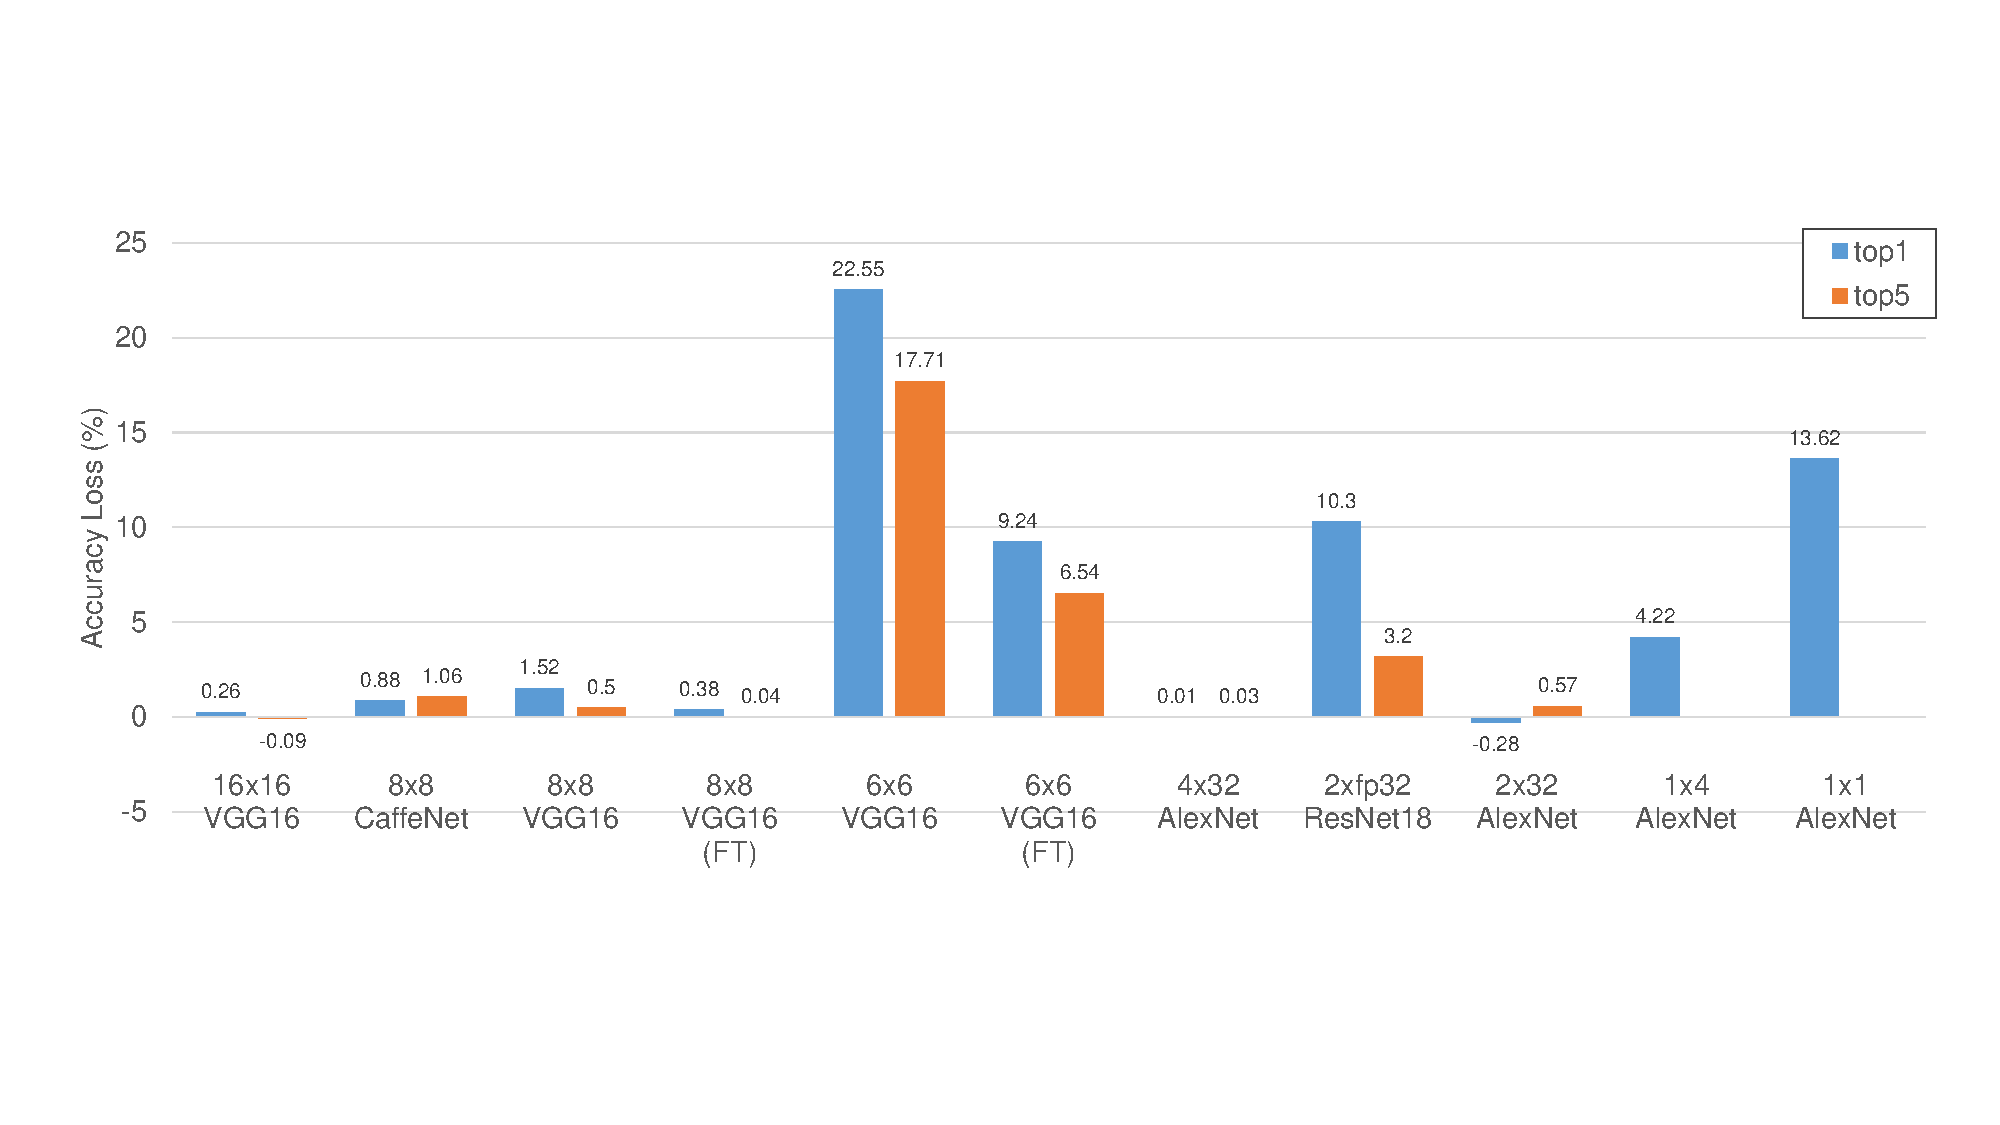
\includegraphics[width=1.0\columnwidth]{fig/quantization.pdf}
    \caption{Comparison between different quantization methods from \cite{qiu2016going, guo2017angel, han2015deep, zhu2016trained, zhou2016dorefa, li2016ternary}.}
    \label{fig:quantization}
\end{figure}

\subsection{Weight Reduction}
Besides narrowing the bit-width of neurons and weights, another method for model compression is to reduce the number of weights. One kind of method is to approximate the weight matrix with a low rank representation. Qiu, et al.~\cite{qiu2016going} compress the weight matrix $W$ of an FC layer with singular value decomposition. An $m\times n$ weight matrix $W$ is replaced by the multiplication of two matrices $A_{m\times p}B_{p\times n}$. For a sufficiently small $p$, the total number of weights is reduced. This work compress the largest FC layer of VGG network to $36\%$ of its original size with $0.04\%$ classification accuracy degradation. Zhang, et al.~\cite{zhang2015efficient} use similar method for convolution layers and takes the effect of the following non-linear layer into the decomposition optimization process. The proposed method achieves $4\times$ speed up on state-of-the-art CNN model targeting at ImageNet, with only $0.9\%$ accuracy loss.

Pruning is another kind of method to reduce the number of weights. This kind of method directly remove the zeros in weights or remove those with small absolute values. The challenge in pruning is how to make more weights zero while keeping the model accuracy. One solution is the application of lasso object function during training. Liu, et al.~\cite{liu2015sparse} apply the spase group-lasso object function on the AlexNet~\cite{krizhevsky2012imagenet} model. $90\%$ weights are removed after training with less than $1\%$ accuracy loss. Another solution is to prune the zero weights during training. Han, et al.~\cite{han2015deep} directly removes the values in network with zero or small absolute value. The left weights are then fine-tuned are training set to recover accuracy. Experimental result on AlexNet show that $89\%$ weights can be removed while keeping the model accuracy.

\section{Hardware Design: Efficient Architecture}\label{sec:hardware}

In this section, we investigate the hardware level techniques used in state-of-the-art FPGA-based neural network accelerator design to achieve high performance and high energy efficiency. We classify the techniques into three levels: computation unit level, loop unrolling level, and system level.

\subsection{Computation Unit Designs}\label{sec:hardware:cu}

Computation unit level design affects the peak performance of the neural network accelerator. The available resource of an FPGA chip is limited. A smaller computation unit design means more computation units and higher peak performance. A carefully designed computation unit array can also increase the working frequency of the system and thus improve peak performance.

\subsubsection{Low Bit-width Computation Unit}\label{sec:hardware:cu:lbu}
Reduce the number of bit-width for computation is a direct way to reduce the size of computation units. The feasibility of using fewer bits comes from the quantization methods as introduced in section~\ref{sec:software:quant}. Most of the state-of-the-art FPGA designs replace the 32-bit floating-point units with fixed-point units. Podili et al.~\cite{podili2017fast} implement 32-bit fixed-point units for the proposed system. 16-bit fixed-point units are widely adopted in \cite{qiu2016going, li2016high, xiao2017exploring, guan2017fp, zhang2016caffeine}. ESE~\cite{han2017ese} adopts 12-bit fixed-point weight and 16-bit fixed-point neurons design. Guo et al.~\cite{guo2017angel} use 8-bit units for their design on embedded FPGA. Recent work is also focusing on extremely narrow bit-width design. Prost-Boucle et al.~\cite{prost2017scalable} implements 2-bit multiplication with 1 LUT for ternary networks. Experiments in \cite{nurvitadhi2016accelerating} show that FPGA implementation of Binarized Neural Network (BNN) outperforms that on CPU and GPU. Though BNN suffers from accuracy loss, many designs explore the benefit of using 1-bit data for computation~\cite{li20177, nakahara2017batch, zhao2017accelerating, umuroglu2017finn, nakahara2017fully, jiao2017accelerating, moss2017high, yang2018fully, ghasemzadehrebnet}.

The designs mentioned above focus on computation units for linear quantization. For non-linear quantization, translating the data back to full precision for computation still costs many resources. Samragh et al.~\cite{samragh2017customizing} propose the factorized coefficients based dot product implementation. As the possible values of weights are quite limited for non-linear quantization, the proposed computation unit accumulates the multipliers for each possible weight value and calculate the result as the weighted sum of the values in look-up tables. In this way, the multiplication needed for one output neuron equals to the number of values in look-up table. The multiplications are replaced by random-addressed accumulations.

Most of the designs use one bit-width through the process of a neural network. Qiu et al.~\cite{qiu2016going} finds that neurons and weights in FC layers can use fewer bits compared with CONV layers while the accuracy is maintained. Heterogeneous computation units are used in the designs of \cite{zhao2017accelerating, guo2017bit}.

The size of computation units of different bit-widths is compared in Table~\ref{tab:mac}. Three kinds of implementations are tested: separate multiplier and adder with logic resource on Xilinx FPGA, multiply-add function with DSP units on Xilinx FPGA, and multiply-add function with DSP units on Altera FPGA. The resource consumption is the synthesis result by Vivado 2018.1 targeting Xilinx XCKU060 FPGA and Quartus Prime 16.0 targeting Altera Arria 10 GX1150 FPGA. The pure logic modules and the floating-point multiply and add modules are generated with IP core. The fixed-point multiply and add modules are implemented with $A*B+C$ in Verilog and automatically mapped to DSP by Vivado/Quartus.

We first give an overview of the size of the computation units by logic-only implementations. By compressing the weights and activations from 32-bit floating-point number to 8-bit fixed-point number, the multiplier and the adder are scaled down to about 1/10 and 1/50 respectively. Using 4-bit or smaller operators can bring further advantage but also incur significant accuracy loss as introduced in section~\ref{sec:software:quant}. 

Recent FPGAs consist of a large number of DSP units, each of which implements hard multiplier, pre-adder and accumulator core. The basic pattern of NN computation, multiplication and sum, also fits into this design. So we also test the multiply and add function implemented with DSP units. Because of the different DSP architectures, we test on both Xilinx and Altera platforms. Compared with the 32-bit floating-point function, fixed-point functions with narrow bit-width still shows an advantage in resource consumption. But for Altera FPGA, this advantage is not obvious because the DSP units natively support floating-point operations. 

Fixed-point functions with 16-or-less-bit fixed-point data are well fit into 1 DSP unit on either Xilinx or Altera FPGA. This shows that quantization hardly benefits the hardware if we use narrower bit-width like 8 or 4 in the aspect of computation. The problem is that the wide multipliers and adders in DSP units are underutilized in these cases. Nguyen et al.~\cite{nguyen2017double} propose the design to implement two narrow bit-width fixed-point multiplication with a single wide bit-width fixed-point multiplier. In this design, two multiplications, $AB$ and $AC$, are executed in the form of $A(B<<k+C)$. If $k$ is sufficiently large, the bits for $AB$ and $AC$ does not overlap in the multiplication result and can be directly separated. The design in~\cite{nguyen2017double} implements two 8-bit multiplications with one $25\times 18$ multiplier, where $k$ is 9. Similar methods can be applied to other bit-width and DSPs.

%\begin{figure}[ht]
%    \centering
%    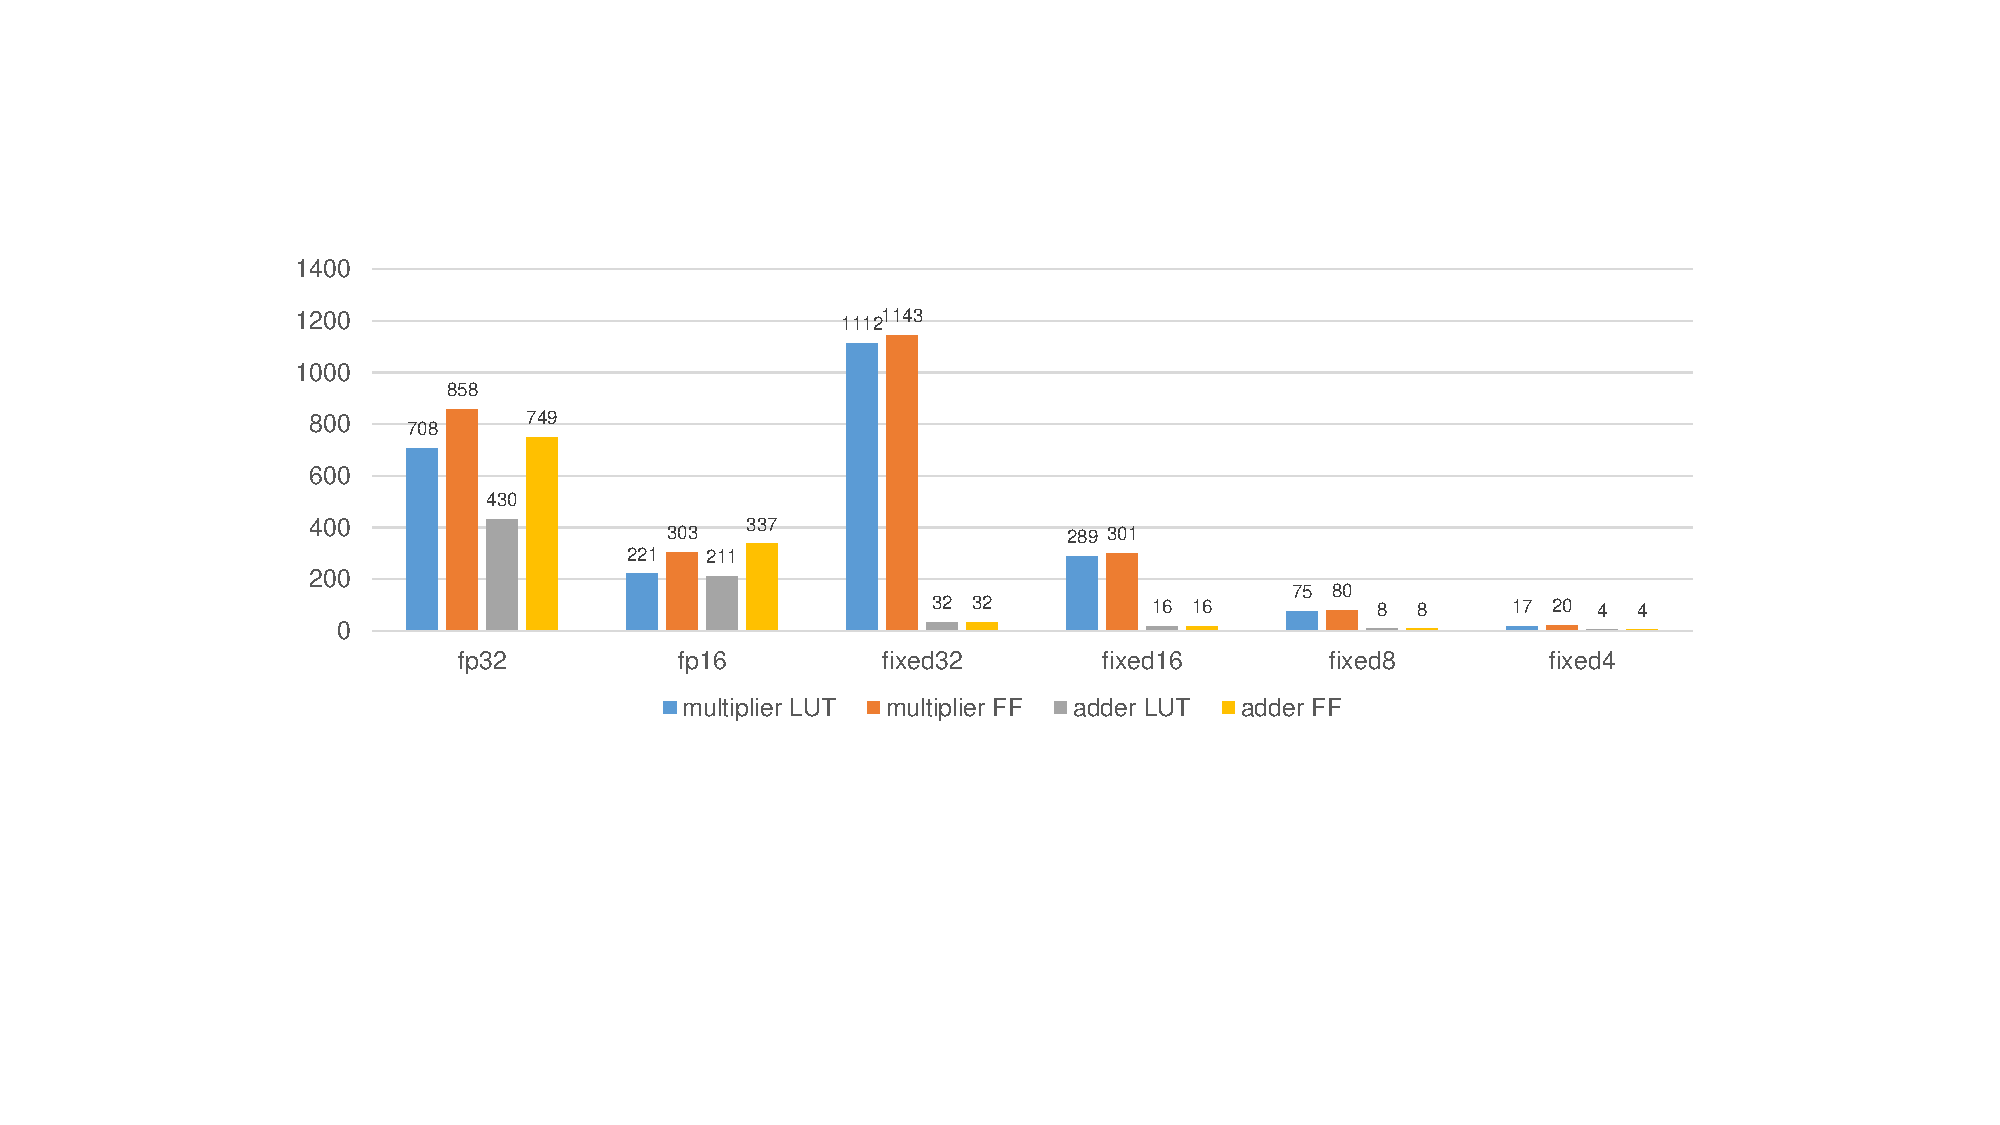
\includegraphics[width=1.0\columnwidth]{fig/mac_util.pdf}
%    \caption{FPGA resource consumption comparison for multiplier and adder with different types of data.}
%    \label{fig:mac_util}
%\end{figure}

% Table generated by Excel2LaTeX from sheet 'Sheet1'
\begin{table}[htbp]
    \centering
    \caption{\rev{FPGA resource consumption comparison for multiplier and adder with different types of data.}}
      \begin{tabular}{|l|r|r|r|r|r|r|r|r|r|} \hline
      \multirow{2}[4]{*}{} & \multicolumn{4}{c|}{Xilinx Logic} & \multicolumn{3}{c|}{Xilinx DSP} & \multicolumn{2}{c|}{Altera DSP} \\ \cline{2-10}         
       & \multicolumn{2}{c|}{multiplier} & \multicolumn{2}{c|}{adder} & \multicolumn{3}{c|}{multiply \& add} & \multicolumn{2}{c|}{multiply \& add} \\ \cline{2-10}
            & \multicolumn{1}{c|}{LUT} & \multicolumn{1}{c|}{FF} & \multicolumn{1}{c|}{LUT} & \multicolumn{1}{c|}{FF} & \multicolumn{1}{c|}{LUT} & \multicolumn{1}{c|}{FF} & \multicolumn{1}{c|}{DSP} & \multicolumn{1}{c|}{ALM} & \multicolumn{1}{c|}{DSP} \\ \hline
      fp32  & 708   & 858   & 430   & 749   & 800   & 1284  & 2     & 1     & 1 \\ \hline
      fp16  & 221   & 303   & 211   & 337   & 451   & 686   & 1     & 213   & 1 \\ \hline
      fixed32 & 1112  & 1143  & 32    & 32    & 111   & 64    & 4     & 64    & 3 \\ \hline
      fixed16 & 289   & 301   & 16    & 16    & 0     & 0     & 1     & 0     & 1 \\ \hline
      fixed8 & 75    & 80    & 8     & 8     & 0     & 0     & 1     & 0     & 1 \\ \hline
      fixed4 & 17    & 20    & 4     & 4     & 0     & 0     & 1     & 0     & 1 \\ \hline
      \end{tabular}
    \label{tab:mac}
  \end{table}
  

\subsubsection{Fast Convolution Method}\label{sec:hardware:cu:fcu}
For CONV layers, the convolution operations can be accelerated by alternative algorithms. Discrete Fourier Transformation (DFT) based fast convolution is widely adopted in digital signal processing. Zhang et al.~\cite{zhang2017frequency} propose a 2D DFT based hardware design for efficient CONV layer execution. For an $F\times F$ filter convolved with $K\times K$ filter, DFT converts the $(F-K+1)^2K^2$ multiplications in the space domain to $F^2$ complex multiplications in the frequency domain. For a CONV layer with $M$ input channel and $N$ output channel, $MN$ times of frequency domain multiplications and $(M+N)$ times DFT/IDFT are needed. The conversion of convolution kernels is once for all. So the domain conversion process is of low cost for CONV layers. This technique does not work for CONV layers with stride>1 or $1\times 1$ convolution. Ding et al.~\cite{ding2017c} suggest that a block-wise circular constraint can be applied to the weight matrix. In this way, the matrix-vector multiplication in FC layers are converted to a set of 1D convolutions and can be accelerated in the frequency domain. This method can also be applied to CONV layers by treating the $K\times K$ convolution kernels as $K\times K$ matrices and is not limited by $K$ or stride.

Frequency domain methods require complex number multiplication. Another kind of fast convolution involves only real number multiplication~\cite{winograd1980arithmetic}. The convolution of a 2D feature map $F_{in}$ with a kernel $K$ using Winograd algorithm is expressed by equation~\ref{eqt:winograd}.
\begin{equation}\label{eqt:winograd}
    F_{out} = A^T[(GF_{in}G^T)\odot(BF_{in}B^T)]A
\end{equation}
$G$, $B$ and $A$ are transformation matrix which only related to the sizes of kernel and feature map. $\odot$ denotes an element-wise multiplication of two matrices. For a $4\times 4$ feature map convolved with a $3\times 3$ kernel, the transformation matrices are described as follows:
\begin{equation*}
    G = \left[
        \begin{array}{ccc}
            1           & 0            & 0           \\
            \frac{1}{2} & \frac{1}{2}  & \frac{1}{2} \\
            \frac{1}{2} & -\frac{1}{2} & \frac{1}{2} \\
            0           & 0            & 1
        \end{array}    
    \right] \quad
    B = \left[
        \begin{array}{cccc}
            1 & 0  & -1 & 0 \\
            0 & 1  & 1  & 0 \\
            0 & -1 & 1  & 0 \\
            0 & 1  & 0  & -1
        \end{array}
    \right] \quad
    A = \left[
        \begin{array}{cc}
            1 & 0  \\
            1 & 1  \\
            1 & -1 \\
            0 & -1 
        \end{array}
    \right]
\end{equation*}
Multiplication with transformation matrices $A, B$ and $G$ induce only a small number of shift and addition because of the special matrix entries. In this case, the number of multiplication is reduced from 36 to 16.The most commonly used Winograd transformation is for $3\times 3$ convolutions in \cite{lu2017evaluating, xiao2017exploring}. 

The theoretical performance gain from fast convolution depends on the convolution size. Limited by the on-chip resource and the consideration of flexibility, current designs are not choosing large convolution sizes. Existing work point out that up to $4\times$ theoretical performance gain can be achieved by fast convolution with FFT~\cite{zhang2017frequency} or Winograd~\cite{lu2017evaluating} with reasonable kernel sizes. Zhuge et al.~\cite{zhuge2018face} even try to use both FFT and Winograd methods in their design to fit different kernel sizes in different layers.

\subsubsection{Frequency Optimization Methods}
All the above techniques introduced targets at increasing the number of computation units within a certain FPGA. Increasing the working frequency of the computation units also improves the peak performance.

Latest FPGAs support 700-900MHz DSP theoretical peak working frequency. But existing designs usually work at 100-400MHz~\cite{qiu2016going, guo2017angel, zhang2016caffeine, ma2017optimizing, zhang2017improving}. As claimed in \cite{wu2017high}, the working frequency is limited by the routing between on-chip SRAM and DSP units. The design in \cite{wu2017high} uses different working frequencies for DSP units and surrounding logic. Neighbor slices to each DSP unit are used as local RAMs to separate the clock domain. The prototype design in \cite{wu2017high} achieves the peak DSP working frequency at 741MHz and 891MHz on FPGA chips of different speed grades. \rev{Xilinx has also proposed the CHaiDNN-v2~\cite{chai_dnn} and xfDNN~\cite{xfdnn} with this technique and achieves up to 700MHz DSP working frequency. Compared with existing designs for which the frequency is within 300MHz, this technique brings at least $2\times$ peak performance gain.}

\subsection{Loop Unrolling Strategies}\label{sec:hardware:lu}
CONV layers and FC layers contribute to most of the computations and storage requirement of a neural network as introduced in section~\ref{sec:preliminary}. We express the CONV layer function in Figure~\ref{fig:cnn_preliminary}(b) as nested loops in Algorithm~\ref{alg:conv}. To make the code clear to read, we merge the loops along $x$ and $y$ directions for feature maps and 2-D convolution kernels respectively. An FC layer can be expressed as a CONV layer with feature map and kernel both of size $1\times 1$. Besides the loops in Algorithm~\ref{alg:conv}, we also call the parallelism of the process of multiple inputs as a batch. As we treat FC layers and CONV layers all as nested loops, the loop unrolling strategy can be applied both in CNN accelerators and RNN accelerators. But as the case for FC layers are rather simple, we tend to use CNN as examples in this section.

\begin{algorithm}  
    \caption{Convolution Layer}
    \label{alg:conv}
    \begin{algorithmic}[1]
        \Require feature map $F_{in}$ of size $M\times Y\times X$; 
                 convolution kernel $Ker$ of size $N\times M\times K\times K$;
                 bias vector $b$ of size $N$ 
        \Ensure  feature map $F_{out}$
        \Function {ConvLayer}{$F_{in}, Ker$}  
            \State Let $F_{out} \gets $ zero array of size $N\times(Y-K+1)\times(X-K+1)$  
            \For{$n=1$; $n<N$; $n++$} \Comment Output channel loop
                \For{$m=1$; $m<M$; $m++$} \Comment Input channel loop
                    \For{each $(y, x)$ within $(Y-K+1, X-K+1)$} \Comment Feature map loop
                        \For{each $(ky, kx)$ within $(K, K)$} \Comment Kernel loop
                            \State $F_{out}[n][y][x] += F_{in}[m][y-ky+1][x-kx+1] * K[n][m][ky][kx]$
                        \EndFor
                    \EndFor
                \EndFor
                \State $F_{out}[n] += b[n]$
            \EndFor
            \State \Return{$F_{out}$}
        \EndFunction  
        
    \end{algorithmic}  
\end{algorithm}

\subsubsection{Choosing Unroll Parameters}

To parallelize the execution of the loops, we unroll the loops and parallelize the process of a certain number of iterations on hardware. The number of the parallelized iterations on hardware is called the unroll parameter. Inappropriate unroll parameter selection may lead to serious hardware underutilization. Take a single loop as an example. Suppose the trip count of the loop is $M$ and the parallelism is $m$. The utilization ratio of the hardware is limited by $m/M\lceil M/m\rceil$. If $M$ is not divisible by $m$, then the utilization ratio is less than 1. For processing an NN layer, the total utilization ratio will be the product of the utilization ratio on each of the loops.

%Take an example of three nested loops as shown in Figure~\ref{fig:unrolling}. The big cube denotes all the operations within the loops. The length of each edge denotes the trip count of each loop. The small cube denotes the unrolled kernel. The hardware process all the operations of a small cube in parallel. To finish the workload, the hardware computes the small cubes one by one.  Figure~\ref{fig:unrolling}(a) shows an appropriate set of unroll parameters. But for Figure~\ref{fig:unrolling}(b), the red part of some of the small cubes are out of the big cube, which means the hardware is wasted.

%\begin{figure}[ht]
%    \centering
%    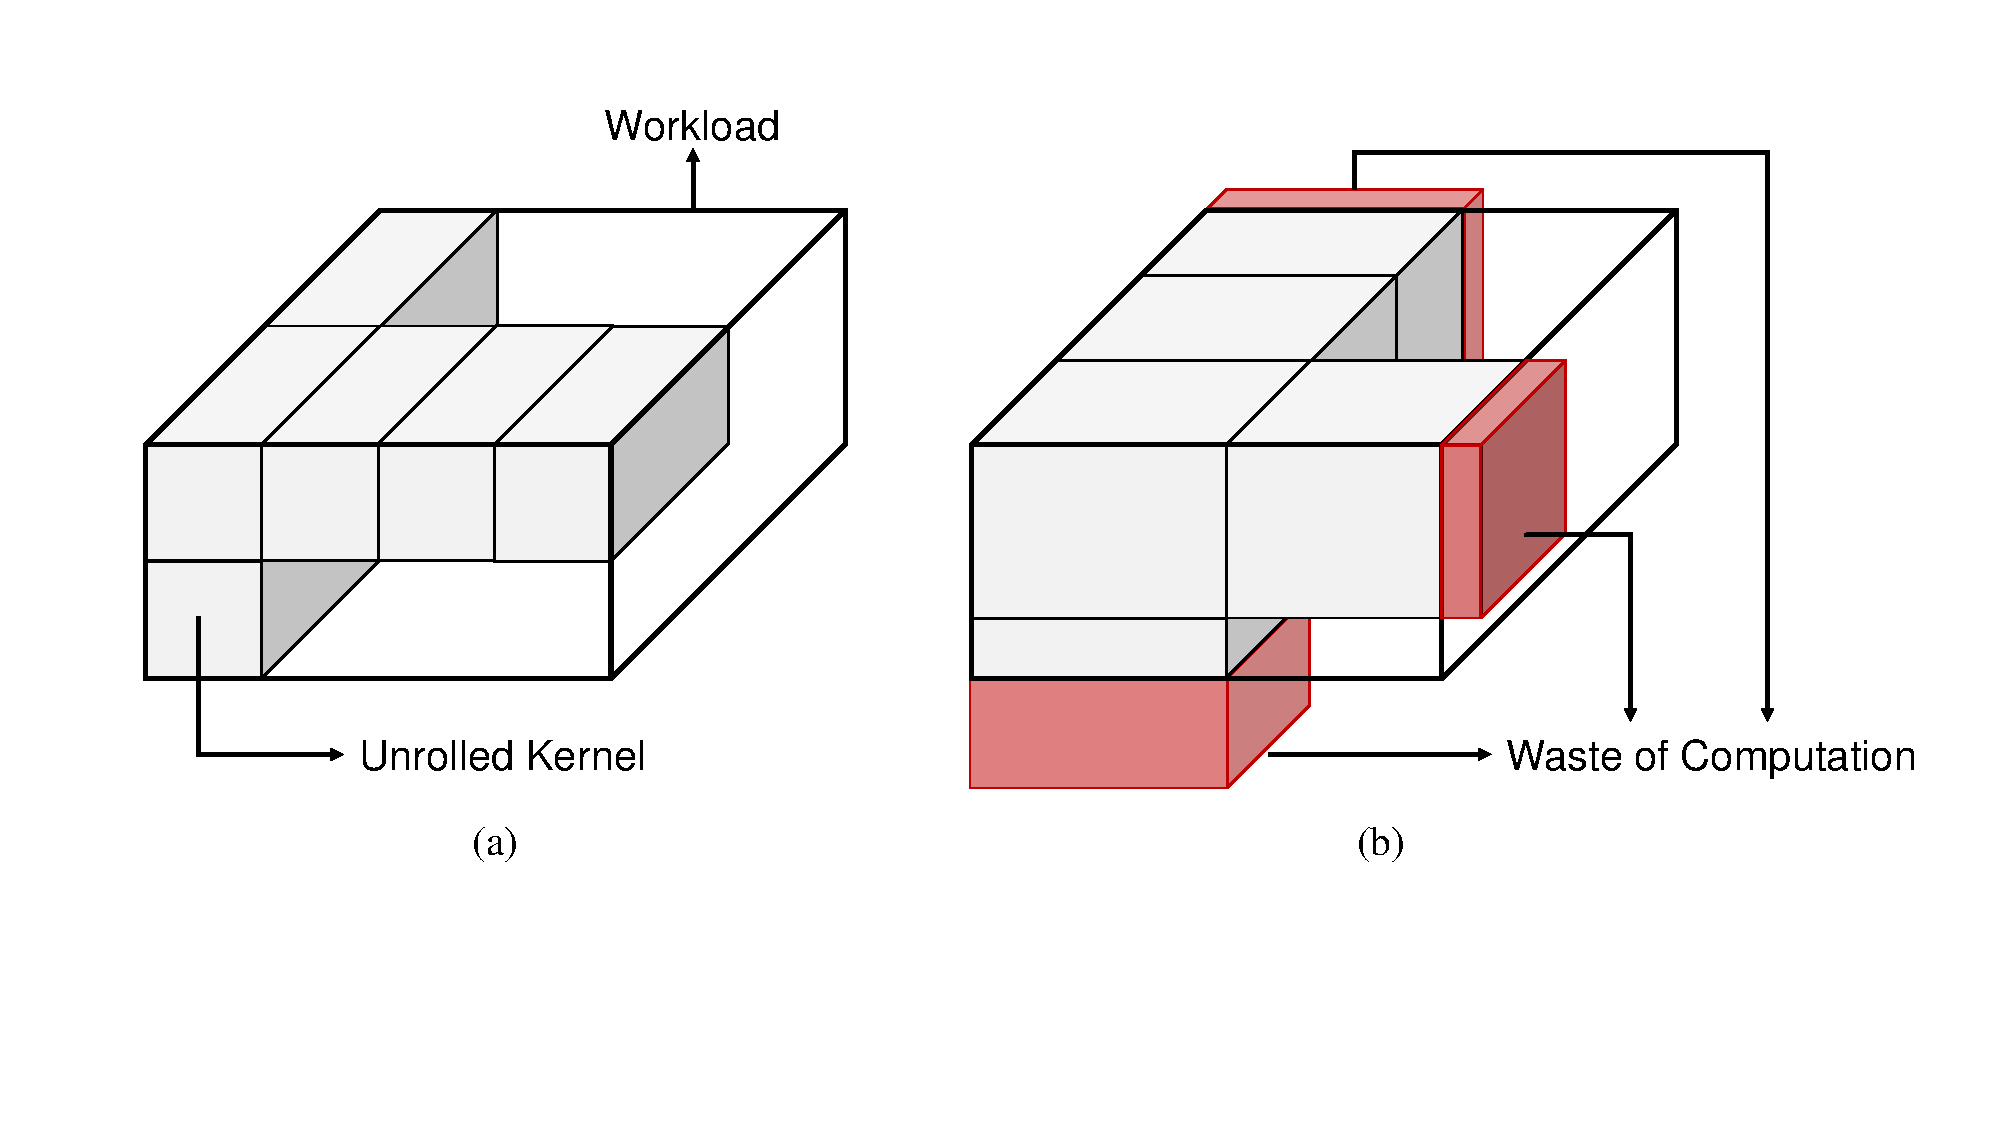
\includegraphics[width=0.8\columnwidth]{fig/unrolling.pdf}
%    \caption{Comparison between appropriate and inappropriate loop unroll parameters. (a) Appropriate parameters. (b) Inappropriate parameters.}
%    \label{fig:unrolling}
%\end{figure}

For a CNN model, the loop dimension varies greatly among different layers. For a typical network used on ImageNet classification like ResNet~\cite{he2016deep}, the channel numbers vary from 3 to 2048; the feature map sizes vary from $224\times 224$ to $7\times 7$, the convolution kernel sizes vary from $7\times 7$ to $1\times 1$. Besides the underutilization problem, loop unrolling also affect the datapath and on-chip memory design. Thus loop unrolling strategy is a key feature for a neural network accelerator design. 

Various work are proposed focusing on how to choose the unroll parameters. Zhang et al.~\cite{zhang2015optimizing} propose the idea of unrolling the input channel and output channel loops and choose the optimized unroll parameter by design space exploration. Along these two loops, there is no input data cross-dependency between neighboring iterations. So no multiplexer is needed to route data from the on-chip buffer to computation units. But the parallelism is limited as $7\times 64=448$ multipliers. For larger parallelism, this solution is easy to suffer from the underutilization problem. Ma et al.~\cite{ma2017optimizing} further extends the design space by allowing parallelism on the feature map loop. The parallelism reaches $1\times 16\times 14\times 14=3136$ multipliers. A shift register structure is used to route feature map pixels to the computation units.

The kernel loop is not chosen in the above work because kernel sizes vary greatly. Motamedi et al~\cite{motamedi2016design} use kernel unrolling on AlexNet. Even with $3\times 3$ unrolling for the $11\times 11$ and $5\times 5$ kernels, the overall system performance still reaches 97.4\% of its peak performance for the convolution layers. For certain networks like VGG~\cite{simonyan2014very}, only $3\times 3$ convolution kernels are used. Another reason to unroll kernel loop is to achieve acceleration with fast convolution algorithms. Design in \cite{zhang2017frequency} implements fully parallelized frequency domain multiplication on $4\times 4$ feature map and $3\times 3$ kernel. Lu et al.~\cite{lu2017evaluating} implement Winograd algorithm on FPGA with a dedicated pipeline for equation~\ref{eqt:winograd}. The convolution of a $6\times 6$ feature map with a $3\times 3$ kernel is fully parallelized.

The above solutions are only for a single layer. But there is hardly a one-size-fits-all solution for a whole network, especially when we need high parallelism. Designs in \cite{li2016high, liu2016automatic, zhang2018dnnbuilder} propose fully pipelined structures with each layer a pipe stage. As each layer is executed with an independent part of the hardware and each part is small, loop unrolling method can be easily chosen. This method is memory consuming because ping-pong buffers are needed between adjacent layers for the feature maps. Agressive design with binarized weights~\cite{yang2018fully} can fit into FPGA better. Design in \cite{zhang2016energy} is similar but implemented on FPGA clusters to resolve the scalability problem. Shen et al.~\cite{shen2016overcoming} and Lin et al.~\cite{lin2018lcp} group the layers of a CNN by the loops' trip count and map each group onto one hardware module. These solutions can be treated as unrolling the batch loop because different inputs are processed in parallel on different layer pipeline stages. The design in \cite{lu2017evaluating} implements parallelized batch both within a layer and among different layers. 

Most of the current designs follow one of the above methods for loop unrolling. A special kind of design is for sparse neural networks. Han et al.~\cite{han2017ese} propose the ESE architecture for sparse LSTM network acceleration. Unlike processing a dense network, all the computation units will not work synchronously. This causes difficulty in sharing data between different computation units. ESE implements only the output channel (the output neurons of the FC layers in LSTM) loop unrolling within a layer to simplify hardware design and parallelize batch process.

\subsubsection{Data Transfer and On-chip Memory Design}

Besides the high parallelism, the on-chip memory system should efficiently offer the necessary data to each computation units every cycle. To implement high parallelism, neural network accelerators usually reuse data among a large number of computation units. Simply broadcasting data to different computation units leads to large fan-out and high routing cost and thus reduce the working frequency. Wei et al.~\cite{wei2017automated} use the systolic array structure in their design. The shared data are transferred from one computation unit to the next in a chain mode. So the data is not broadcasted, and only local connections between different computation units are needed. The drawback is the increase in latency. The loop execution order is scheduled accordingly to cover the latency. Similar designs are adopted in~\cite{aydonat2017opencl, ma2017optimizing}. 

For software implementation on GPU, the im2col function is commonly used to map 2D convolution as a matrix-vector multiplication. This method incurs considerable data redundancy and can hardly be applied to the limited on-chip memory of FPGAs. Qiu et al.~\cite{qiu2016going} uses the line buffer design to achieve the $3\times 3$ sliding window function for 2-d convolution with only two lines of duplicated pixels. 

\subsection{System Design}\label{sec:hardware:sys}

A typical FPGA-based neural network accelerator system is shown in Figure~\ref{fig:sys}. The logic part of the whole system is denoted by the blue boxes. The host CPU issues workload or commands to the FPGA logic part and monitors its working status. On the FPGA logic part, a controller is usually implemented to communicate with the host and generates control signals to all the other modules on FPGA. The controller can be an FSM or an instruction decoder. The on the fly logic part is implemented for certain designs if the data loaded from external memory needs preprocess. This module can be data arrangement module, data shifter~\cite{qiu2016going}, FFT module~\cite{zhang2017frequency}, etc. The computation units are as discussed in section~\ref{sec:hardware:cu} and section~\ref{sec:hardware:lu}. As introduced in section~\ref{sec:preliminary:fpga}, on-chip SRAM of an FPGA chip is too limited compared with the large NN models. So for common designs, a two-level memory hierarchy is used with DDR and on-chip memory. 

\begin{figure}[t]
    \centering
    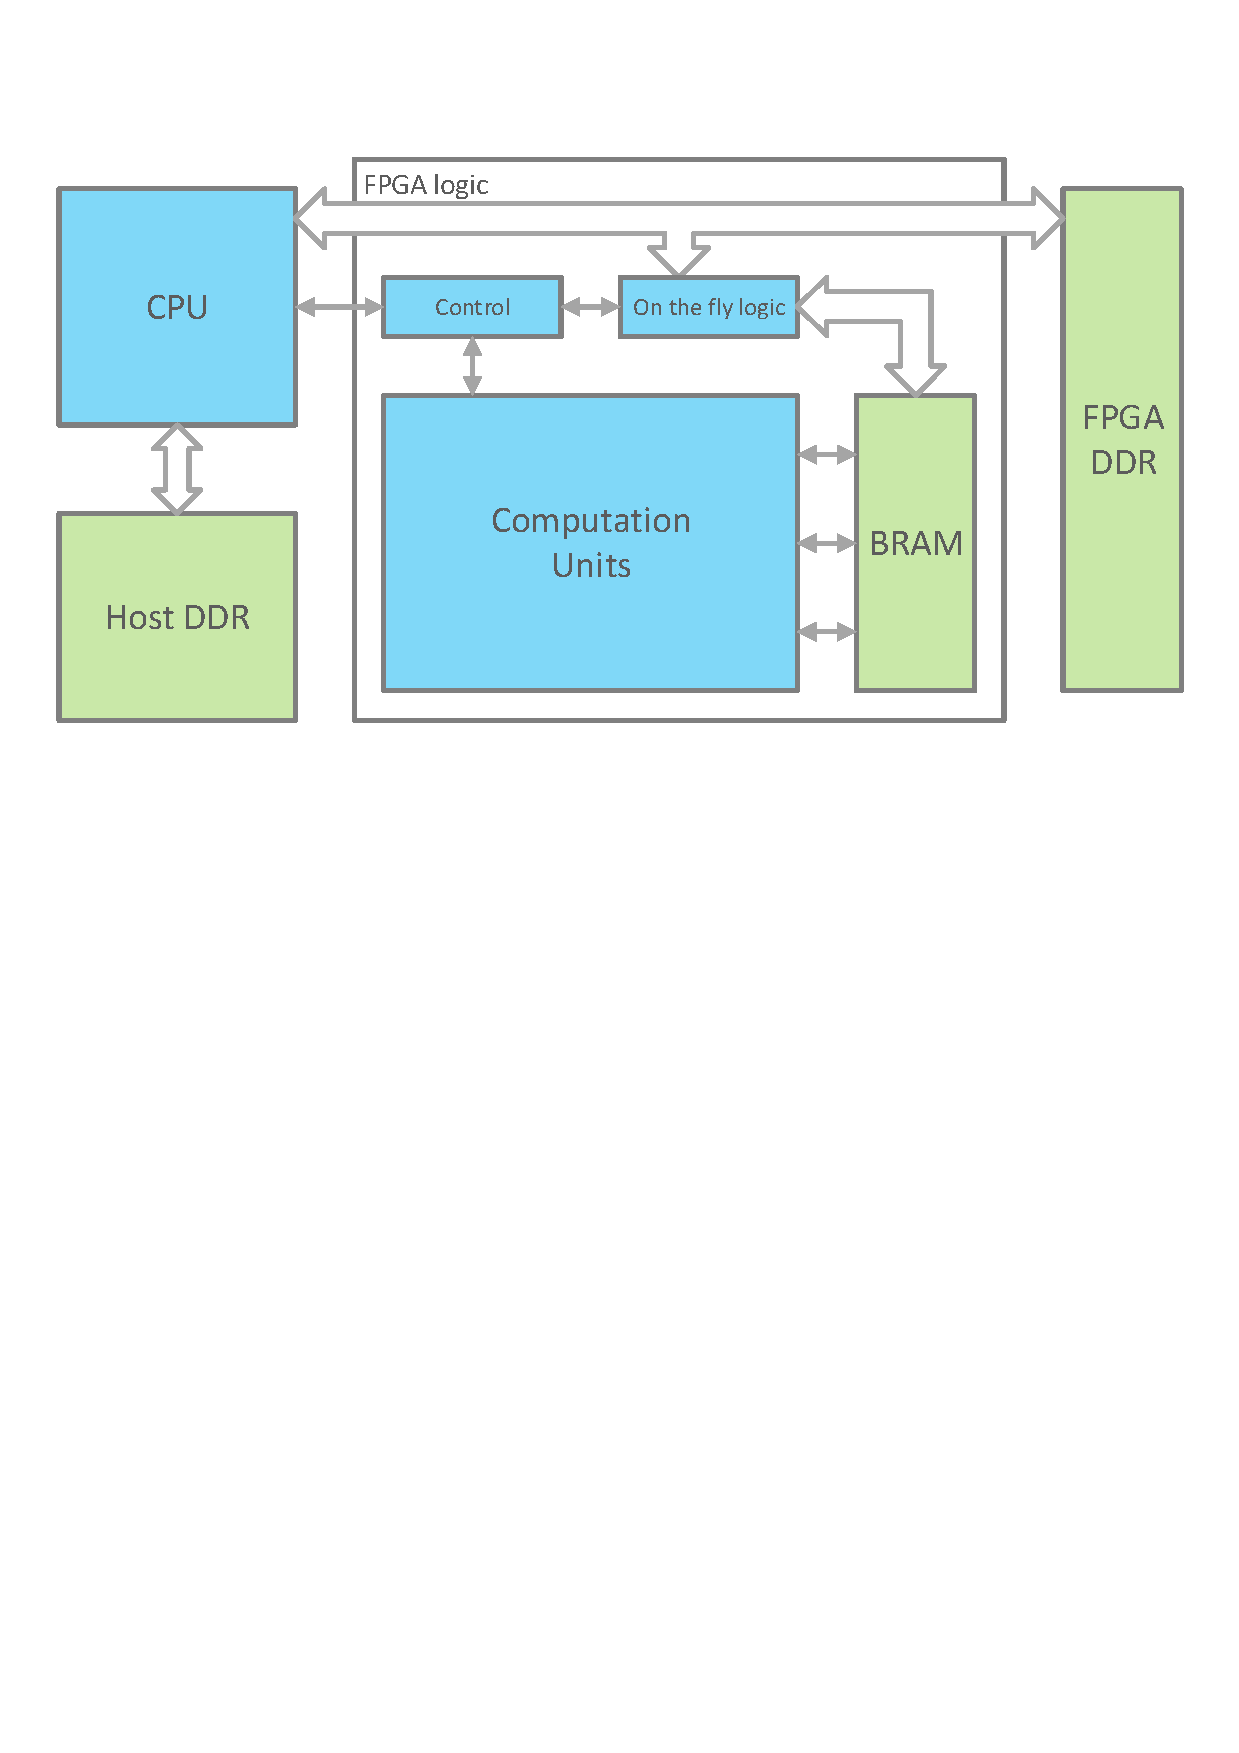
\includegraphics[width=0.8\columnwidth]{fig/sys.pdf}
    \caption{Block graph of a typical FPGA-based neural network accelerator system}
    \label{fig:sys}
\end{figure}

\subsubsection{\rev{Roofline Model}} From the system level, the performance of a neural network accelerator is limited by two factors: the on-chip computation resource and the off-chip memory bandwidth. Various researches have been proposed to achieve the best performance within a certain off-chip memory bandwidth. Zhang et al.~\cite{zhang2015optimizing} introduce the roofline model in their work to analyze whether a design is memory bounded or computation bounded. An example of a roofline model is shown in Figure~\ref{fig:roofline}.

\begin{figure}[h]
    \centering
    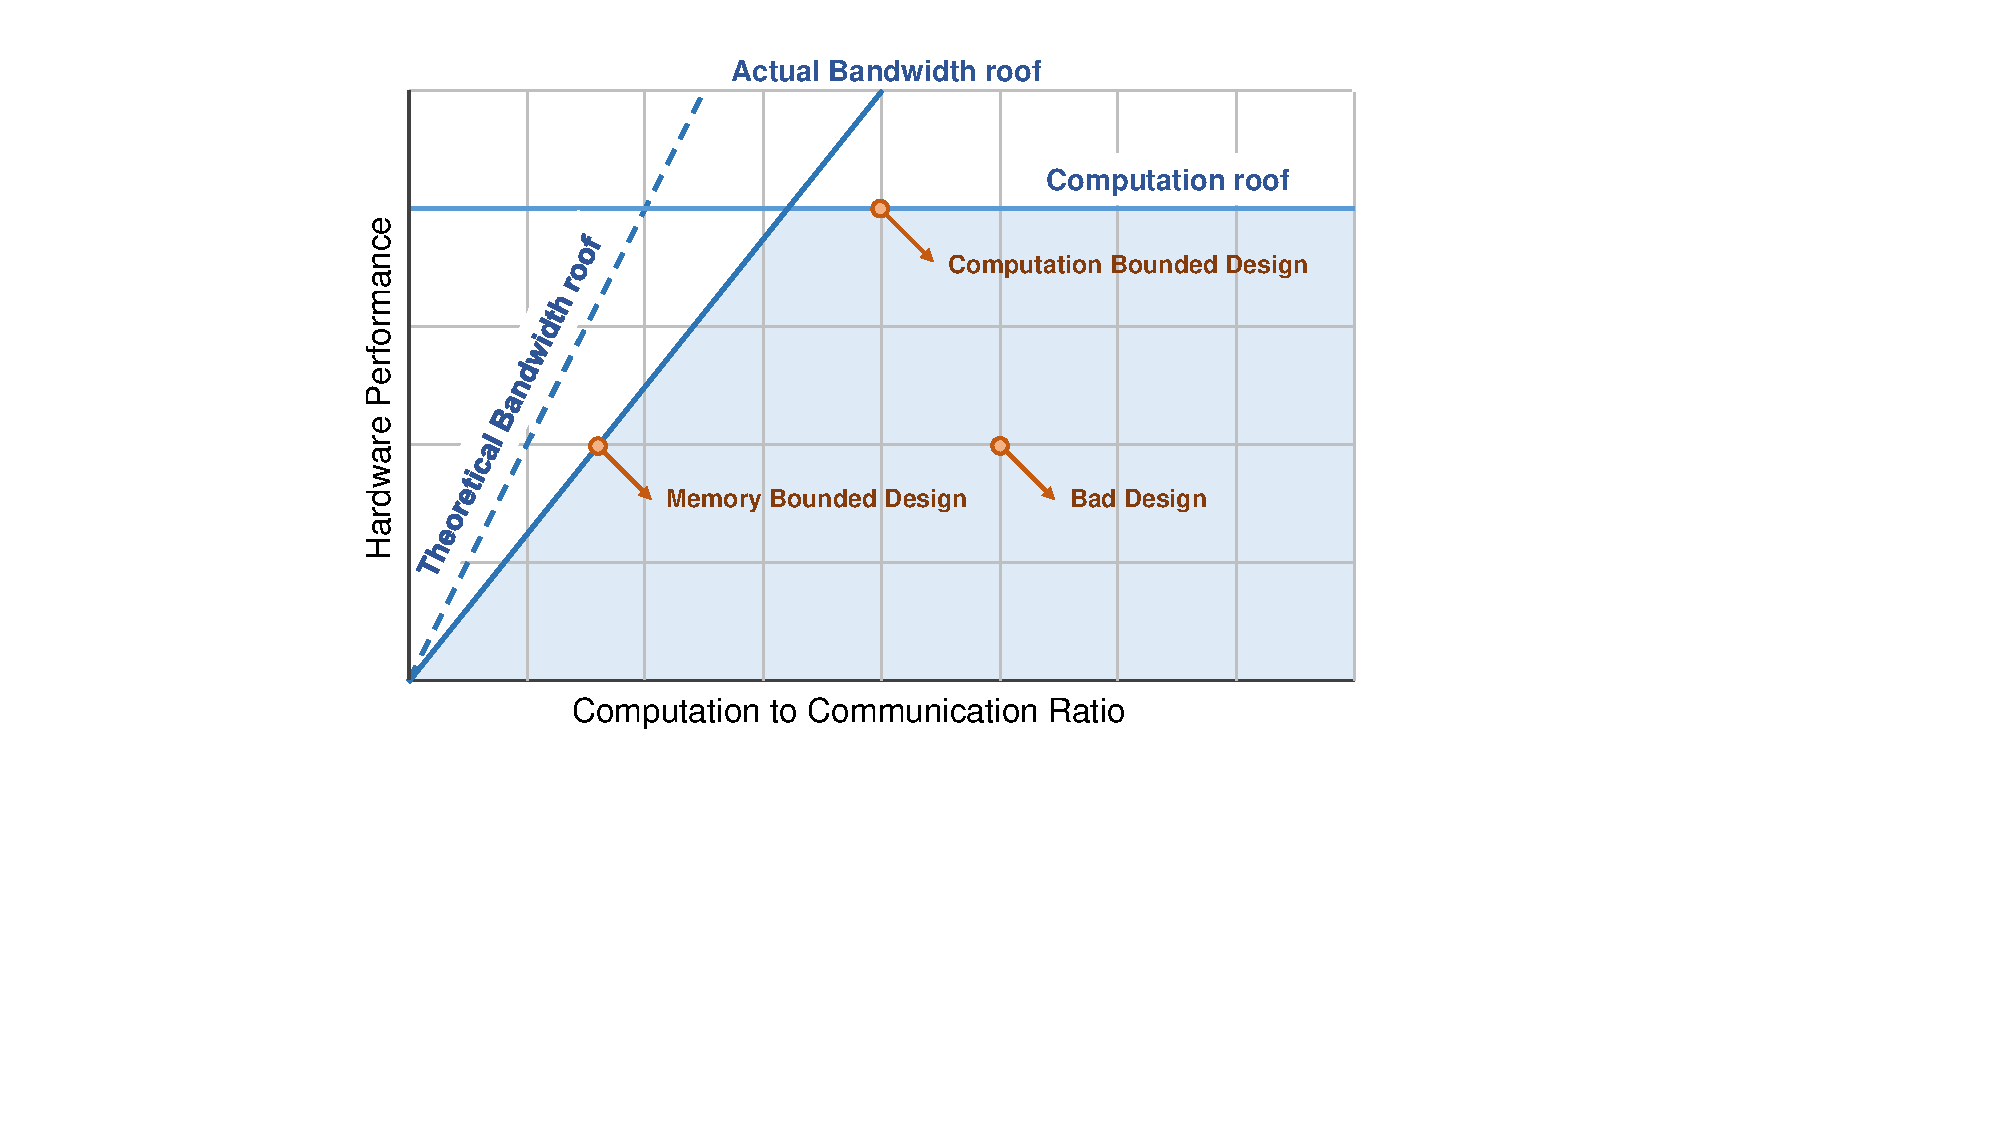
\includegraphics[width=0.6\columnwidth]{fig/roofline.pdf}
    \caption{An example of the roofline model. The shaded part denotes the valid design space given bandwidth and resource limitation.}
    \label{fig:roofline}
\end{figure}

The figure uses the computation to communication (CTC) ratio as the $x$-axis and hardware performance as the $y$-axis. CTC is the number of operations that can be executed with a unit size of memory access. Each hardware design can be treated as a point in the figure. So $y/x$ equals to the bandwidth requirement of the design. The available bandwidth of a target platform is limited and can be described as the theoretical bandwidth roof in Figure~\ref{fig:roofline}. But the actual bandwidth roof is below the theoretical roof because the achievable bandwidth of DDR depends on the data access pattern. Sequential DDR access achieves much higher bandwidth than random access. The other roof is the computation roof, which is limited by the available resource on FPGA.

\subsubsection{\rev{Loop Tiling and Interchange}} A higher CTC ratio means the hardware is more likely to achieve the computation bound. Increasing the CTC ratio also reduce DDR access, which significantly saves energy according to~\cite{vlsi_energy}. In section~\ref{sec:hardware:lu}, we have discussed the loop unrolling strategies to increase the parallelism while reducing the waste of computation for a certain network. When the loop unrolling strategy is decided, the scheduling of the rest part of the loops decides how the hardware can reuse data with on-chip buffer. This involves loop tiling and loop interchange strategy.

Loop tiling is a higher level of loop unrolling. All the input data of a loop tile will be stored on-chip, and the loop unrolling hardware kernel works on these data. A larger loop tile size means that each tile will be loaded from external memory to on-chip memory fewer times. Loop interchange strategy decides the processing order of the loop tiles. External memory access happens when the hardware is moving from one tile to the next. Neighboring tile may share a part of data. For example in a CONV layer, neighboring tile can share input feature map or the weights. This is decided by the execution order of the loops. 

In ~\cite{zhang2015optimizing, ma2017optimizing}, design space exploration is done on all the possible loop tiling sizes and loop orders. Many designs also explore the design space with some of the loop unrolling, tiling and loop order is already decided~\cite{motamedi2016design, qiu2016going}. Shen et al.~\cite{shen2017escher} also discuss the effect of batch parallelism over the CTC for different layers. This is a loop dimension not focused on in previous work.

All the above work give one optimized loop unrolling strategy and loop order for a whole network. Guo et al.~\cite{guo2017angel} implements flexible unrolling and loop order configuration for different layers with an instruction interface. The data arrangement in on-chip buffers is controlled through instructions to fit with different feature map sizes. This means the hardware can always fully utilize the on-chip buffer to use the largest tiling size according to on-chip buffer size. This work also proposes the "back and forth" loop execution order to avoid total on-chip data refresh when an innermost loop finishes.

\subsubsection{\rev{Cross-Layer Scheduling}} Alwani et al.~\cite{alwani2016fused} address the external memory access problem by fusing two neighboring layers together to avoid the intermediate result transfer between the two layers. This strategy helps reduce 95\% off-chip data transfer with extra 20\% on-chip memory cost. Even software program gains $2\times$ speedup with this scheduling strategy. Yu et al.~\cite{Yu2017Instruction} realize this idea on a single-layer accelerator design by modifying the order of execution through an instruction interface.

\subsubsection{\rev{Regularize Data Access Pattern}} Besides increasing CTC, increasing the actual bandwidth roof helps improve the achievable performance with a certain CTC ratio. This is achieved by regularizing the DDR access pattern. The common feature map formats in the external memory include $NCHW$ or $CHWN$, where $N$ means the batch dimension, $C$ means the channel dimension, $H$ and $W$ means the feature map $y$ and $x$ dimension. Using any of these formats, a feature map tile may be cut into small data blocks stored in discontinuous addresses. Guan~\cite{guan2017fp} suggest that a channel-major storage format should be used for their design. This format avoids data duplication while long DDR access burst is ensured. Qiu et al.~\cite{qiu2016going} propose a feature map storage format that arranges the $H\times W$ feature map into $(HW/rc)$ tile blocks of size $r\times c$. So the write burst size can be increased from $c/2$ to $rc/2$.


\bibliographystyle{ACM-Reference-Format}
\bibliography{ref}

\end{document}
